% Lacrosse Scoop: RL-Learned Trajectory Transferred Open-Loop to a Real Robot
%
% This is a self-contained article template meant to be uploaded to Overleaf
% (create a Blank Project there, then upload this file plus anything you put
% in figures/). It compiles standalone with pdfLaTeX.

\documentclass[11pt]{article}

\usepackage[margin=1in]{geometry}
\usepackage{graphicx}
\usepackage{amsmath}
\usepackage{booktabs}
\usepackage{hyperref}
\usepackage{caption}
\usepackage{xcolor}

\newcommand{\todo}[1]{\textcolor{red}{\textbf{[TODO: #1]}}}

\title{Learning to Scoop: A Sparse/Dense-Shaped RL Policy for a 3-DOF\\
Manipulator, Transferred Open-Loop to Real Hardware}
\author{\todo{your name}}
\date{\today}

\begin{document}
\maketitle

\begin{abstract}
We train a reinforcement learning policy in Isaac Lab to control a 3-DOF
chassis-mounted manipulator (one prismatic base joint, two revolute arm joints)
to scoop a lacrosse ball off the ground into a stick pocket and bring it to rest.
The policy is trained with PPO using a dense, phase-structured reward covering
approach, contact, scooping, holding, and deceleration behavior. We then extract
the joint-space trajectory ($x, q_1, q_2$) of a single successful simulated
episode and replay it \emph{open-loop} on the physical robot, with no perception,
no closed-loop control, and no policy inference on hardware. With the ball placed
approximately 1\,m in front of the robot, this blind replay scoops the ball
successfully in roughly half of the attempts, demonstrating that the learned
motion is physically realizable on real hardware despite the total absence of a
closed feedback loop at test time.
\end{abstract}

\section{Problem Statement}
\label{sec:problem}

Scooping a small, fast-rolling ball off the ground with a rigid stick-and-pocket
end-effector is a contact-rich manipulation problem: the controller must (1)
approach the ball's position while it may still be moving, (2) time an arm sweep
so the pocket intercepts the ball from below rather than pushing it away, and (3)
absorb the resulting momentum and hold the ball still, all without letting the
end-effector collide with the ground. Classical trajectory-planning approaches
struggle here because the contact dynamics between the ball and the concave
pocket geometry are difficult to model accurately in closed form.

We ask two questions:
\begin{enumerate}
  \item Can a model-free RL policy, trained purely in simulation with a shaped
        reward, learn this scoop-and-hold behavior on a 3-DOF manipulator?
  \item If we take a single successful simulated trajectory and replay it
        open-loop on the real robot --- i.e.\ we throw away the policy, the
        ball-position sensing, and the closed control loop, and keep only the
        joint-angle time series --- does the motion still work in the real
        world?
\end{enumerate}
Question 2 is deliberately the simplest possible sim-to-real test: any success
rate above chance is evidence that the \emph{shape} of the learned motion, not
just the policy that produced it, is physically valid.

\section{Method}
\label{sec:method}

\subsection{Robot and Task}

The robot is a 3-DOF mobile manipulator: a chassis that slides along $x$, a
shoulder joint $q_1$, and an elbow joint $q_2$, with a lacrosse-stick pocket
rigidly attached at the end effector (Fig.~\ref{fig:robot}, \todo{insert a
photo or CAD render of the real robot here}). The pocket position is obtained
in closed form via forward kinematics:
\begin{align}
  \theta &= q_1 + q_2 \\
  x_{\text{pocket}} &= x + L\sin q_1 - c_x \cos\theta - c_z \sin\theta \\
  z_{\text{pocket}} &= z_0 + L\cos q_1 + c_x \sin\theta - c_z \cos\theta
\end{align}
with arm length $L = 0.30$\,m, shoulder height $z_0 = 0.15$\,m, and pocket
offset constants $c_x = 0.323$\,m, $c_z = 0.07$\,m.

The task: starting from the home pose $x = q_1 = q_2 = 0$, a $32$\,mm-radius,
$145$\,g ball spawns on the ground $0.8$--$1.0$\,m in front of the chassis. The
robot must move the pocket to intercept the ball, lift it, and hold it
near-stationary.

\begin{figure}[h]
  \centering
  % \includegraphics[width=0.6\textwidth]{figures/robot.png}
  \fbox{\parbox{0.6\textwidth}{\centering\vspace{2cm}\todo{robot photo / render}\vspace{2cm}}}
  \caption{The 3-DOF chassis--shoulder--elbow manipulator used for both
  simulation and hardware experiments.}
  \label{fig:robot}
\end{figure}

\subsection{Simulation and RL Formulation}

Training uses Isaac Lab / PhysX at 1200\,Hz physics with a 60\,Hz policy rate
(20 substeps per action). The observation is an 11-dimensional vector: the
three joint positions and velocities, the ball position relative to the pocket
($\Delta x, \Delta z$), a ball-orientation proxy, and ball velocity
($v_x, v_z$) --- no temporal history or recurrent state. The action is
3-dimensional and bounded to $[-1, 1]$: the first component is a chassis
\emph{acceleration} command (integrated into a velocity target, capped at
$\pm 2$\,m/s), and the remaining two are direct velocity targets for the
shoulder and elbow. Using acceleration rather than velocity for the chassis
forces the policy to actively decelerate rather than snap to a target; a
curriculum shrinks the maximum per-step acceleration from
$0.3\,\text{m/s}^2$ to $\tfrac{1}{60}\,\text{m/s}^2$ over the first
$\sim$130k policy steps, progressively demanding finer control.

An episode terminates on success (ball held near-stationary, $< 0.5$\,m/s,
while in contact, for 5 consecutive steps), on an unsafe pocket-to-ground
height, on the ball leaving the workspace, on the ball being flung too high,
or on a 10\,s timeout.

\subsection{Reward Design}
\label{sec:reward}

The reward is a dense, phase-structured sum, deliberately designed so each
phase of the task (approach $\to$ contact $\to$ scoop $\to$ hold $\to$
decelerate) has its own shaping term, gated so that later-phase terms don't
create bad gradients early in the episode. Let $d_x, d_z$ be the ball-to-pocket
offsets, $F$ the measured end-effector--ball contact force, and $v_{\text{ball}}$
the ball's speed.

\begin{align}
r_{\text{chassis}} &= 0.8 \cdot \max(\dot{x}\cdot(-\mathrm{sign}\,d_x),\,0)\cdot\mathbb{1}[|d_x| > 0.35] \\
r_{x} &= 2.0 \cdot e^{-3|d_x|} \\
r_{z} &= 1.0 \cdot e^{-3|d_z|}\cdot\mathbb{1}[|d_x| < 0.35] \\
r_{\text{contact}} &= 5.0 \cdot \mathrm{clip}(F / 10\text{N},\,0,\,1) \\
r_{\text{lift}} &= 5.0 \cdot \max(z_{\text{ball}} - r_{\text{ball}},\,0)/r_{\text{ball}} \\
r_{\text{scoop}} &= 8.0 \cdot \mathbb{1}[\text{contact}]\cdot\mathbb{1}[z_{\text{ball}} < 2.5\,r_{\text{ball}}]\cdot\mathrm{clip}(\dot{q}_2/2.0,\,0,\,1) \\
r_{\text{hold}} &= 10.0 \cdot \mathbb{1}[\text{contact}]\cdot\mathbb{1}[z_{\text{ball}} > 2.5\,r_{\text{ball}}] \\
r_{\text{combo}} &= 0.2 \cdot \min(\text{streak}/5,\,1) \\
r_{\text{vel-inv}} &= 2.0 \cdot \mathbb{1}[\text{holding}] \,/\, (v_{\text{ball}} + 0.05) \\
r_{\text{decel}} &= 30.0 \cdot e^{-v_{\text{ball}}/0.5}\cdot\mathbb{1}[z_{\text{ball}} > 2.5\,r_{\text{ball}}] \\
r_{\text{safety}} &= -8.0 \cdot \max(z_{\text{warn}} - z_{\text{pocket}},\,0) \\
r_{\text{crash}} &= -50 \cdot \mathbb{1}[\text{head-ground termination}] \\
r_{\text{alive}} &= 0.005 \\[4pt]
r_t &= r_{\text{chassis}} + r_x + r_z + r_{\text{contact}} + r_{\text{lift}} + r_{\text{scoop}}
       + r_{\text{hold}} + r_{\text{combo}} + r_{\text{vel-inv}} + r_{\text{decel}}
       + r_{\text{safety}} + r_{\text{crash}} + r_{\text{alive}}
\end{align}

Two design choices are worth calling out. First, $r_{\text{chassis}}$ and
$r_z$ are gated by proximity in $x$, specifically to prevent two reward hacks
observed in earlier iterations: rushing the chassis through the ball to farm
approach reward, and dropping the arm toward the ground before the chassis has
arrived. Second, an earlier version of this environment used one-shot
milestone bonuses (contact / lift / hold / near-stationary-hold, awarded once
each) with no success termination; this caused episodes to always run the
full 600-step horizon regardless of outcome, destabilizing the value function
and causing the policy to collapse after $\sim$50k steps. Replacing the
milestones with the dense, continuously-available terms above and adding an
explicit success termination fixed this.

\subsection{Training}

We use PPO (skrl implementation) with a shared 2-layer MLP backbone
($11 \to 256 \to 128$, ELU activations, $\sim$36.5k parameters) with separate
linear policy and value heads. Key hyperparameters: 256 parallel environments,
32-step rollouts, 8 epochs $\times$ 8 minibatches per update, discount
$\gamma = 0.99$, GAE $\lambda = 0.95$, KL-adaptive learning rate starting at
$3\times10^{-4}$, PPO clip $0.2$, entropy coefficient $0.01$, running
observation/value normalization. The policy is trained from scratch for
400{,}000 policy steps ($\approx$102M environment transitions).

\subsection{Sim-to-Real Transfer Protocol}

Rather than deploying the policy network to hardware, we take the simplest
possible transfer path: motion replay. During a simulated rollout with the
ball spawned $\sim$1\,m in front of the robot, we log the full joint-space
trajectory $(x(t), q_1(t), q_2(t))$ at 60\,Hz from episode start to the instant
the success condition fires. This fixed time series --- with no ball-position
feedback, no contact sensing, and no policy inference --- is then sent
directly as a joint reference to the real robot's controllers, with a real
lacrosse ball placed at the same approximate starting distance
($\sim$1\,m) in front of the physical robot.

\section{Results}
\label{sec:results}

\subsection{Simulation}

\todo{Report a proper held-out success rate here if you re-run evaluation ---
the informal training telemetry for this checkpoint shows mean episode length
converging near the 600-step timeout rather than terminating early on success,
suggesting the sim success rate is likely modest, not the near-100\% reported
for other reward variants of this task. State the actual measured number once
you have it (e.g.\ from N frozen-policy rollouts).}

Figure~\ref{fig:traj} shows one successful simulated trajectory: the ball
leaves the ground and crosses the success-height threshold within about
0.1\,s of first lifting off, with post-contact ball velocity peaking near
2\,m/s before settling.

\begin{figure}[h]
  \centering
  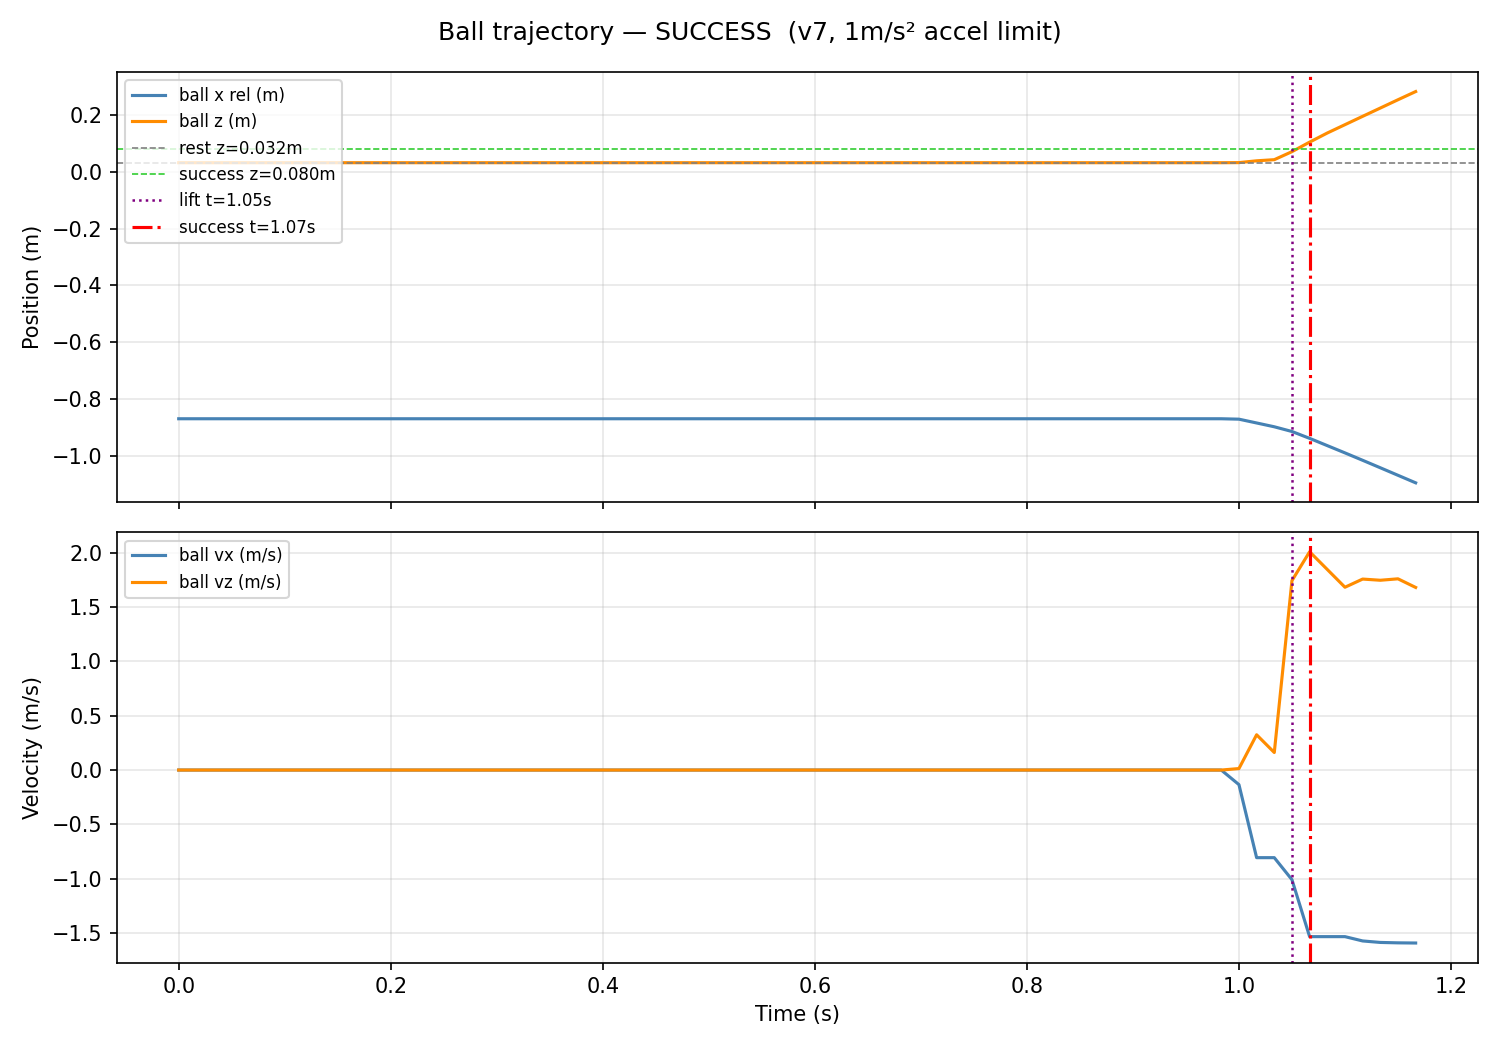
\includegraphics[width=0.8\textwidth]{figures/ball_trajectory.png}
  \caption{Simulated ball position and velocity vs.\ time for one successful
  scoop episode. The ball lifts off the ground at $t\approx1.05$\,s and
  crosses the success-height threshold at $t\approx1.07$\,s.}
  \label{fig:traj}
\end{figure}

\subsection{Open-Loop Real-Robot Replay}

Replaying the extracted $(x, q_1, q_2)$ trajectory open-loop on the physical
robot, with the ball placed $\sim$1\,m in front of the robot at the start of
each trial, produced a successful scoop in approximately \textbf{half of the
attempts} (\todo{report exact N and success count once you have logged
trials, e.g.\ ``6/12''}).

\begin{table}[h]
\centering
\begin{tabular}{lll}
\toprule
Setting & Feedback used & Outcome \\
\midrule
Simulation (trained policy) & full state, closed-loop & \todo{sim success rate} \\
Real robot (open-loop replay) & none (fixed motion) & $\approx$50\% scoop success \\
\bottomrule
\end{tabular}
\caption{Simulation vs.\ real-robot outcomes. The real-robot condition uses no
perception or feedback at all --- it is a blind replay of one recorded
simulated trajectory.}
\end{table}

\section{Discussion}
\label{sec:discussion}

A $\sim$50\% success rate with zero feedback on hardware is, in one sense, a
strong result: it shows the learned motion --- the specific timing of chassis
approach, arm sweep, and deceleration --- transfers to the real robot's
dynamics well enough to work without any correction. In another sense, it is
an expected ceiling: the policy was trained on a single simulated ball spawn
distribution with ground-truth state and no domain randomization, so the
\emph{fixed} motion it produced is only correct for one particular ball
position and one particular (simulated) set of contact dynamics. On hardware,
ball placement, rolling drift, surface friction, and actuator response
(latency, backlash) vary from trial to trial, and an open-loop replay has no
mechanism to correct for any of it. The failure mode we would expect --- and
which matches informal observation --- is the pocket arriving at the ball's
simulated position while the real ball has rolled or bounced slightly
elsewhere.

This suggests two directions to raise the real-world success rate without
changing the underlying task: (1) train with domain randomization over ball
mass/friction/restitution and, ideally, injected observation noise, so the
learned trajectory is less brittle to the exact contact dynamics assumed in
sim; and (2) close the loop on hardware --- estimate real ball position (e.g.\
depth camera or marker tracking) and run the trained policy's inference at
control time instead of replaying a fixed motion, so the controller can react
to trial-to-trial variation instead of assuming it away.

\section{Conclusion}
\label{sec:conclusion}

We trained a dense-reward PPO policy to scoop a ball with a 3-DOF manipulator
in simulation, and showed that a single successful trajectory extracted from
that policy transfers to real hardware via pure open-loop joint replay, with
roughly 50\% success and no perception or feedback of any kind at test time.
This is best read as a proof of concept that the learned motion is physically
realizable, and as a baseline to beat with closed-loop, randomization-hardened
deployment in future work.

\end{document}
